\documentclass[11pt]{article}

\usepackage[margin=1in]{geometry}
\usepackage[T1]{fontenc}
\usepackage{lmodern}
\usepackage{microtype}
\usepackage{xcolor}
\usepackage{hyperref}
\usepackage{listings}
\usepackage{tikz}
\usetikzlibrary{arrows.meta,positioning,shapes.geometric}

\hypersetup{
  colorlinks=true,
  linkcolor=blue!60!black,
  urlcolor=blue!60!black
}

\lstdefinelanguage{TDSTR}{
  morekeywords={system,vars,vars*,domain,domain*,init,action,next,invariant,property,
    proc,source,set,not,eventually,if,then,assign,to,as,equals,unchanged*,
    forall,exists,and,or,alternate-scenarios,implies,in,quote,same,unchanged},
  sensitive=true,
  morecomment=[l]{\#},
  morestring=[b]"
}

\lstset{
  basicstyle=\ttfamily\small,
  keywordstyle=\color{blue!65!black}\bfseries,
  commentstyle=\color{green!35!black},
  stringstyle=\color{red!55!black},
  showstringspaces=false,
  columns=fullflexible,
  keepspaces=true,
  frame=single,
  breaklines=true
}

\title{TDSTR Reference Manual\\\large Tcl Front End and Tooling}
\author{Sambuddha Majumder and Jayanta Majumder}
\date{\today}

\begin{document}
\maketitle
\tableofcontents

\section{Purpose and Scope}

TDSTR is the Tcl-shaped front end for the \texttt{dstr} finite-state modelling
prototype.  It uses Tcl's command and brace syntax to describe the same model
concepts as DSTR and CDSTR: finite variables, domains, initial states, actions,
the next-state relation, invariants, and reachability-style properties.  The
TDSTR compiler emits normalized JSON for the common checker and graph tools.

TDSTR is a good fit when a Tcl interpreter is available and the model benefits
from Tcl's lightweight command language, \texttt{proc} definitions, and
\texttt{source}d helper files.

\section{Pipeline}

\begin{center}
\resizebox{\textwidth}{!}{%
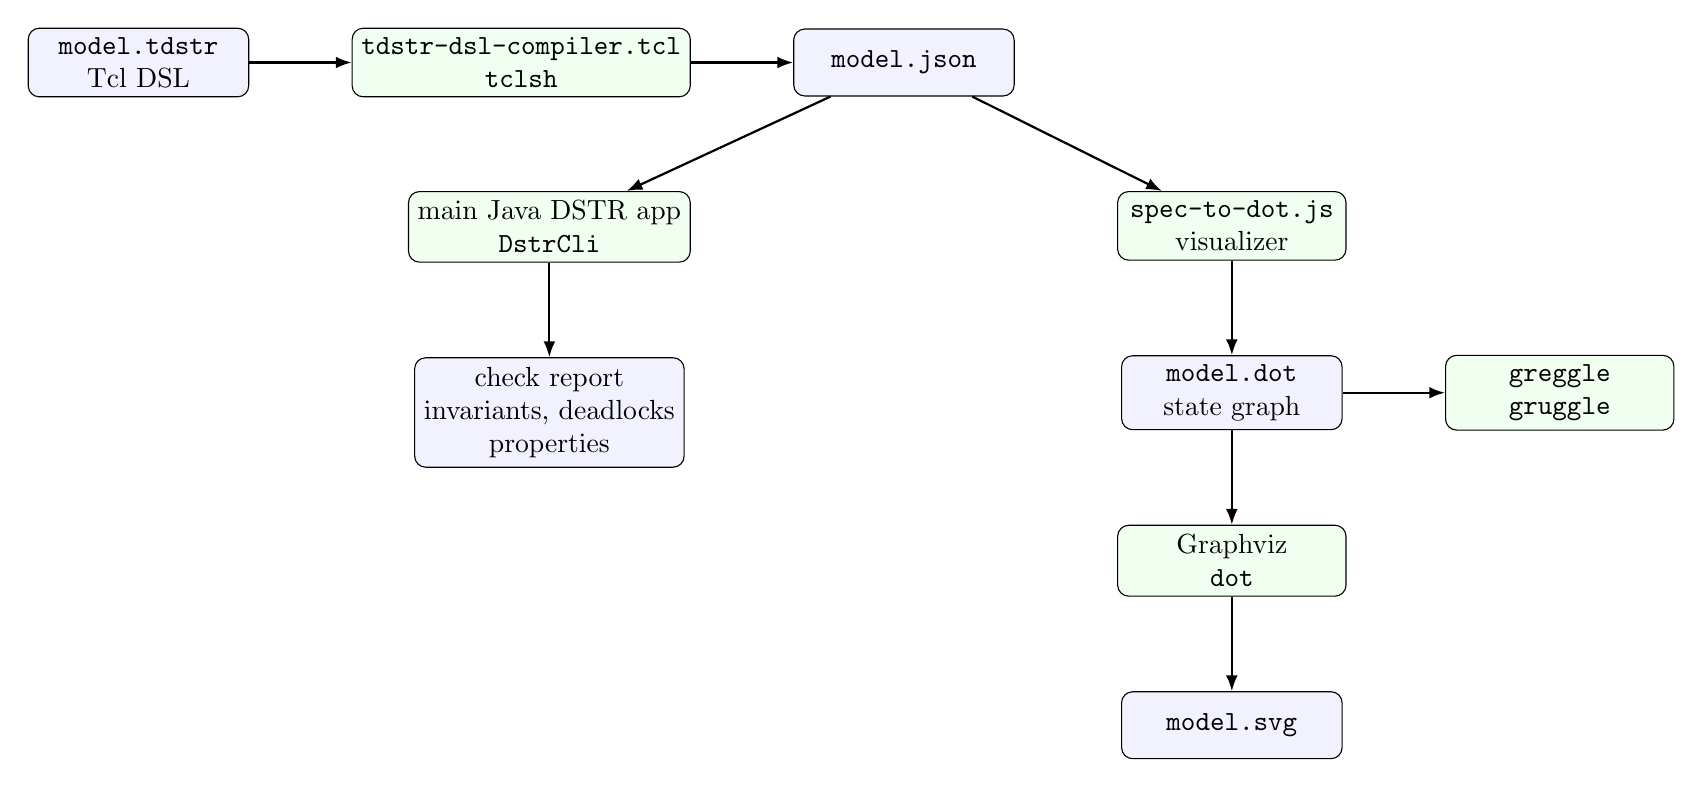
\begin{tikzpicture}[
  node distance=1.2cm and 1.3cm,
  box/.style={draw, rounded corners, align=center, minimum width=2.8cm,
    minimum height=0.85cm, fill=blue!5},
  tool/.style={draw, rounded corners, align=center, minimum width=2.9cm,
    minimum height=0.85cm, fill=green!6},
  arr/.style={-{Latex[length=2mm]}, thick}
]
\node[box] (src) {\texttt{model.tdstr}\\Tcl DSL};
\node[tool, right=of src] (compiler) {\texttt{tdstr-dsl-compiler.tcl}\\\texttt{tclsh}};
\node[box, right=of compiler] (json) {\texttt{model.json}};
\node[tool, below left=of json] (checker) {main Java DSTR app\\\texttt{DstrCli}};
\node[box, below=of checker] (report) {check report\\invariants, deadlocks\\properties};
\node[tool, below right=of json] (dot) {\texttt{spec-to-dot.js}\\visualizer};
\node[box, below=of dot] (dotfile) {\texttt{model.dot}\\state graph};
\node[tool, below=of dotfile] (gv) {Graphviz\\\texttt{dot}};
\node[box, below=of gv] (svg) {\texttt{model.svg}};
\node[tool, right=of dotfile] (gg) {\texttt{greggle}\\\texttt{gruggle}};
\draw[arr] (src) -- (compiler);
\draw[arr] (compiler) -- (json);
\draw[arr] (json) -- (checker);
\draw[arr] (checker) -- (report);
\draw[arr] (json) -- (dot);
\draw[arr] (dot) -- (dotfile);
\draw[arr] (dotfile) -- (gv);
\draw[arr] (dotfile) -- (gg);
\draw[arr] (gv) -- (svg);
\end{tikzpicture}
}
\end{center}

The Tcl compiler is a front end.  Its JSON output should normally be passed to
the root Java DSTR application, \texttt{org.dstr.cli.DstrCli}, for actual model
checking.  The DOT/SVG path is the visualization path: useful for inspecting
small graphs, debugging transitions, and preparing diagrams.  The generated
\texttt{.dot} graph can also be used as input to \texttt{greggle} and
\texttt{gruggle} for graph interrogation and manipulation.

\section{Command Reference}

\subsection{Compile a File}

Run the compiler directly with Tcl:

\begin{lstlisting}[language=bash]
tclsh scripts/tdstr-dsl-compiler.tcl \
  tdstr-testsuite/light-switch.tdstr \
  target/light-switch.json
\end{lstlisting}

PowerShell:

\begin{lstlisting}[language=bash]
tclsh scripts\tdstr-dsl-compiler.tcl `
  tdstr-testsuite\light-switch.tdstr `
  target\light-switch.json
\end{lstlisting}

\subsection{Compile a Directory}

\begin{lstlisting}[language=bash]
tclsh scripts/tdstr-dsl-compiler.tcl tdstr-testsuite target/tdstr-json
\end{lstlisting}

Every \texttt{.tdstr} file in the input directory is compiled to a corresponding
\texttt{.json} file in the output directory.

\subsection{Run the Java Model Checker}

After compiling to JSON, run the main Java checker from the repository root:

\begin{lstlisting}[language=bash]
mvn exec:java -Dexec.args="target/light-switch.json"
gradle run --args="target/light-switch.json"
\end{lstlisting}

The checker parses the JSON emitted by TDSTR, enumerates the finite state
space, computes reachable states from \texttt{init} through \texttt{next},
checks invariants, reports deadlock counterexample paths, and evaluates
\texttt{eventually} properties as existential reachability summaries.  Use this
path for the authoritative pass/fail checking result.

\subsection{Generate SVG}

\begin{lstlisting}[language=bash]
./tdstr-to-svg.sh tdstr-testsuite/light-switch.tdstr
./tdstr-to-svg.sh tdstr-testsuite/bakery-3proc.tdstr --max-states 500
\end{lstlisting}

\begin{lstlisting}[language=bash]
.\tdstr-to-svg.bat tdstr-testsuite\light-switch.tdstr
.\tdstr-to-svg.bat tdstr-testsuite\bakery-3proc.tdstr --max-states 500
\end{lstlisting}

The wrapper accepts \texttt{input.tdstr} or \texttt{input.json}.  It writes
adjacent \texttt{.json}, \texttt{.dot}, and \texttt{.svg} files.  It is meant
for graph inspection and does not replace the Java model-checking CLI.  The
\texttt{.svg} is the visual rendering; the \texttt{.dot} graph is also suitable
as input to \texttt{greggle} or \texttt{gruggle}.

\subsection{Graph Options}

\begin{description}
\item[\texttt{--all-states}] Include unreachable states.
\item[\texttt{--rankdir TB}] Draw top-to-bottom.  Use \texttt{LR} for
  left-to-right.
\item[\texttt{--max-states N}] Truncate very large universes.
\item[\texttt{--compact}] Force compact graph labels.
\item[\texttt{--no-legend}] Omit compact graph legend.
\end{description}

\section{Tcl Source Model}

A TDSTR file is a Tcl script evaluated in an isolated namespace.  The compiler
installs DSL commands such as \texttt{system}, \texttt{vars}, \texttt{domain},
and \texttt{action} into that namespace.  Ordinary Tcl \texttt{proc}
definitions may appear before a \texttt{system}, and helper files may be loaded
with \texttt{source}.  Relative \texttt{source} paths are resolved against the
current \texttt{.tdstr} file's directory.

Use braces to prevent early Tcl substitution in model expressions:

\begin{lstlisting}[language=TDSTR]
action turn-on {= light off} {= light+ on}
\end{lstlisting}

Use command substitution deliberately when invoking helper procedures:

\begin{lstlisting}[language=TDSTR]
action p1-a0 {= p1pc a0} {= p1pc+ a1} {*}[unchanged p2pc c1 c2 turn]
\end{lstlisting}

\section{System Form}

\begin{lstlisting}[language=TDSTR]
system light-switch {
    vars light
    domain light off on
    init {= light off}
    action turn-on {= light off} {= light+ on}
    action turn-off {= light on} {= light+ off}
    next {or @turn-on @turn-off}
    invariant type-ok {in light {set off on}}
    property eventually-on {eventually {= light on}}
}
\end{lstlisting}

\subsection{Clauses}

\begin{description}
\item[\texttt{vars v...}] Declare variables.
\item[\texttt{vars* sep \{a...\} * \{b...\}}] Declare product variables by
  joining each pair with \texttt{sep}.
\item[\texttt{domain v value...}] Declare a finite domain for one variable.
\item[\texttt{domain* pattern value...}] Apply a domain to all declared
  variables matching a Tcl glob pattern.
\item[\texttt{init expr...}] Define initial-state predicate.
\item[\texttt{action name expr...}] Define a named transition predicate.
\item[\texttt{next expr...}] Define next-state relation, usually action refs.
\item[\texttt{invariant name expr...}] Check a predicate on reachable states.
\item[\texttt{property name expr...}] Summarize a property such as
  \texttt{eventually}.
\end{description}

Multiple body expressions in a clause are combined as \texttt{and}.

\section{Atoms and References}

\begin{description}
\item[Current variable] A declared name such as \texttt{pc}.
\item[Next variable] A declared name with trailing \texttt{+}, such as
  \texttt{pc+}.
\item[Action reference] A token beginning with \texttt{@}, such as
  \texttt{@turn-on}, in a \texttt{next} expression.
\item[String literal] An undeclared word such as \texttt{idle}, \texttt{OPEN},
  or \texttt{CANCELLED}.
\item[Numeric literal] Integers and floating point tokens.
\item[Boolean literal] \texttt{true}, \texttt{false}, \texttt{t}, and
  \texttt{nil}.
\item[Quoted literal] \texttt{\{quote foo\}} forces a literal.
\end{description}

\section{Expression Reference}

\subsection{Logic}

\begin{lstlisting}[language=TDSTR]
{and {= pc idle} {= lock free}}
{or @enter @exit}
{not {= pc cs}}
{implies {= pc cs} {= lock held}}
\end{lstlisting}

\subsection{Comparison and Arithmetic}

\begin{lstlisting}[language=TDSTR]
{= count 0}
{!= mem 0}
{< ticket other-ticket}
{<= hr 12}
{= count+ {+ count 1}}
{= remaining+ {- remaining 1}}
\end{lstlisting}

\subsection{Sets and Membership}

\begin{lstlisting}[language=TDSTR]
domain pc idle trying cs
invariant type-ok {in pc {set idle trying cs}}
\end{lstlisting}

\subsection{Quantifiers}

\begin{lstlisting}[language=TDSTR]
invariant known-owner {
    forall {p in {set p1 p2}}
        {in p {set p1 p2}}
}

property owner-can-be-p1 {
    eventually {exists {p in {set p1 p2}} {= p p1}}
}
\end{lstlisting}

\subsection{Reachability-Style Temporal Form}

\begin{lstlisting}[language=TDSTR]
property p1-can-reach-cs {eventually {= p1pc cs}}
\end{lstlisting}

The current checker treats this as reachability, not fairness-based temporal
logic.

\section{Transition Sugar}

\subsection{Assignments}

\begin{lstlisting}[language=TDSTR]
{= light+ on}
{assign on to light}
{set light as on}
\end{lstlisting}

All three assert equality between the next state of \texttt{light} and
\texttt{on}.

\subsection{Equality Alias}

\begin{lstlisting}[language=TDSTR]
{equals p_settlement_state OPEN}
\end{lstlisting}

is equivalent to:

\begin{lstlisting}[language=TDSTR]
{= p_settlement_state OPEN}
\end{lstlisting}

\subsection{Guarded Transition Cases}

\begin{lstlisting}[language=TDSTR]
{
    if
    {
        {equals p_settlement_state OPEN}
        {equals c1_settlement_state OPEN}
        {equals c2_settlement_state OPEN}
    }
    then
    {
        {assign CANCELLED to p_settlement_state}
        {assign CANCELLED to c1_settlement_state}
        {assign CANCELLED to c2_settlement_state}
    }
}
\end{lstlisting}

The \texttt{if ... then ...} form is a guarded-conjunction shorthand.  It is
equivalent to \texttt{and} of the condition block and the consequence block.
There is no \texttt{else} clause.

\subsection{Frame Conditions}

\begin{lstlisting}[language=TDSTR]
{unchanged* *_market_status *_event_type *_mission_version *_mission_revision}
\end{lstlisting}

The compiler expands all matching declared variables into frame equalities.

\subsection{Alternate Scenarios}

\begin{lstlisting}[language=TDSTR]
{
    alternate-scenarios
    {if {= state OPEN} then {assign CANCELLED to state}}
    {if {= state BOOKED} then {assign state to state}}
}
\end{lstlisting}

\texttt{alternate-scenarios} is a synonym for \texttt{or}.

\section{Built-In Tcl Helpers}

\subsection{\texttt{same}}

\begin{lstlisting}[language=TDSTR]
same pc
\end{lstlisting}

returns:

\begin{lstlisting}[language=TDSTR]
{= pc+ pc}
\end{lstlisting}

\subsection{\texttt{unchanged}}

\begin{lstlisting}[language=TDSTR]
action p1-a0 {= p1pc a0} {= p1pc+ a1} {*}[unchanged p2pc c1 c2 turn]
\end{lstlisting}

\texttt{unchanged} returns a Tcl list of sibling frame-condition expressions.
The Tcl expansion operator \texttt{\{*\}} splices them into the action command.

\subsection{Custom Helpers}

\begin{lstlisting}[language=TDSTR]
proc preservePair {left right} {
    return [list [same $left] [same $right]]
}

system example {
    vars left right
    domain left idle done
    domain right idle done
    init {= left idle} {= right idle}
    action finish-left {= left idle} {= left+ done} {*}[preservePair right right]
    next @finish-left
}
\end{lstlisting}

Since TDSTR is Tcl, helpers can compute and return expression lists.  Keep
helper output in the same brace/list shape that the compiler expects.

\section{Product Variables and Domain Globs}

\begin{lstlisting}[language=TDSTR]
system lifecycle {
    vars* _ {master venue1} * {lifecycle trading_status}
    domain* *_lifecycle NEW ENRICHING READY DISABLED
    domain* *_trading_status NOT_TRADING TRADING PAUSED

    init \
        {equals master_lifecycle ENRICHING} \
        {equals venue1_lifecycle ENRICHING}

    action enrichment-complete \
        {if
            {
                {equals master_lifecycle ENRICHING}
                {equals venue1_lifecycle ENRICHING}
            }
            then
            {
                {assign READY to master_lifecycle}
                {assign READY to venue1_lifecycle}
                {assign NOT_TRADING to master_trading_status}
                {assign NOT_TRADING to venue1_trading_status}
            }}

    next @enrichment-complete
}
\end{lstlisting}

\section{Frame-Only Variable Reduction}

The TDSTR compiler performs a safe post-expansion reduction.  Declared
variables that occur only in conjunctive unchanged/frame clauses are omitted
from the emitted JSON.  This reduces state-space size for models with many
fields that are carried along unchanged.

\begin{center}
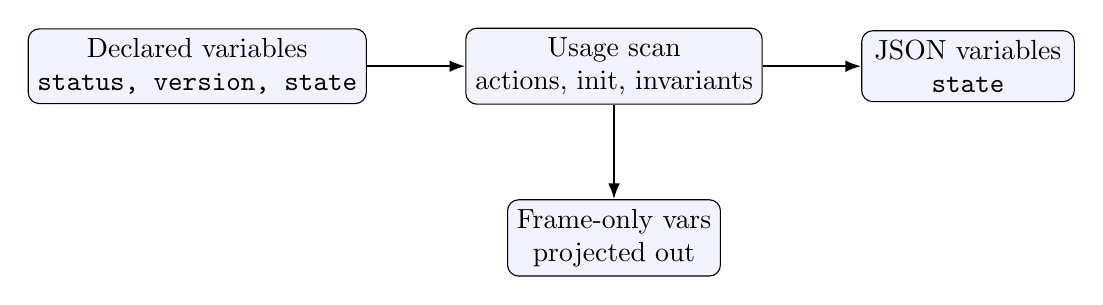
\begin{tikzpicture}[
  node distance=1.2cm and 1.25cm,
  box/.style={draw, rounded corners, align=center, minimum width=2.7cm,
    minimum height=0.85cm, fill=blue!5},
  arr/.style={-{Latex[length=2mm]}, thick}
]
\node[box] (all) {Declared variables\\\texttt{status, version, state}};
\node[box, right=of all] (use) {Usage scan\\actions, init, invariants};
\node[box, right=of use] (keep) {JSON variables\\\texttt{state}};
\node[box, below=of use] (drop) {Frame-only vars\\projected out};
\draw[arr] (all) -- (use);
\draw[arr] (use) -- (keep);
\draw[arr] (use) -- (drop);
\end{tikzpicture}
\end{center}

The graph generator reports projected-out variables in graph labels when that
information is visible through the normalized spec.

\section{State Graph Output}

\begin{center}
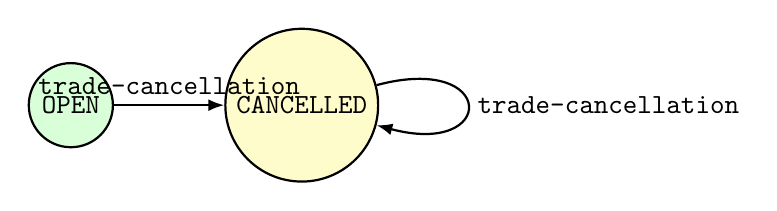
\begin{tikzpicture}[
  node distance=1.4cm,
  state/.style={circle, draw, minimum size=1cm, align=center},
  init/.style={state, fill=green!15, thick},
  dead/.style={state, fill=yellow!20, thick},
  arr/.style={-{Latex[length=2mm]}, thick}
]
\node[init] (open) {\texttt{OPEN}};
\node[dead, right=of open] (cancel) {\texttt{CANCELLED}};
\draw[arr] (open) -- node[above] {\texttt{trade-cancellation}} (cancel);
\draw[arr] (cancel) to[loop right] node[right] {\texttt{trade-cancellation}} (cancel);
\end{tikzpicture}
\end{center}

Green nodes are initial states, amber nodes are deadlocks, and red nodes
indicate invariant failures.  Edges are labelled by actions that justify each
transition.

\section{Full Example: Small Trade Cancellation}

\begin{lstlisting}[language=TDSTR]
system trade-cancellation-parent-children-small {
    vars* _ {p c1 c2} * {market_status settlement_state settlement_version settlement_revision event_type}

    domain* *_market_status MATCHED
    domain* *_settlement_state OPEN RELEASED BOOKED CANCELLED
    domain* *_event_type INSTRUCTION_ACKED
    domain* *_mission_version 1
    domain* *_mission_revision 1

    init \
        {equals p_settlement_state OPEN} \
        {equals c1_settlement_state OPEN} \
        {equals c2_settlement_state OPEN}

    action trade-cancellation \
        {unchanged* *_market_status *_event_type *_mission_version *_mission_revision} \
        {
            alternate-scenarios
            {
                if
                {
                    {equals p_settlement_state OPEN}
                    {equals c1_settlement_state OPEN}
                    {equals c2_settlement_state OPEN}
                }
                then
                {
                    {assign CANCELLED to p_settlement_state}
                    {assign CANCELLED to c1_settlement_state}
                    {assign CANCELLED to c2_settlement_state}
                }
            }
        }

    next @trade-cancellation
}
\end{lstlisting}

\section{Practical Modelling Notes}

\begin{itemize}
\item Use braces for DSL expressions so Tcl does not substitute variables or
  commands too early.
\item Use \texttt{@action} for TDSTR action references.  The lispy
  \texttt{\$action} convention is not used in TDSTR.
\item Use \texttt{\{*\}[helper ...]} when a helper returns multiple sibling
  expressions.
\item Be explicit about frame conditions.  Unconstrained next-state variables
  create extra successor states.
\item Use \texttt{domain*} and \texttt{unchanged*} together for large product
  models.
\item Use \texttt{--max-states} while visualizing large state spaces.
\end{itemize}

\section{Checklist}

\begin{enumerate}
\item Write a \texttt{system name \{...\}} block.
\item Declare variables with \texttt{vars} or \texttt{vars*}.
\item Provide domains with \texttt{domain} or \texttt{domain*}.
\item Define \texttt{init}.
\item Define transition \texttt{action} clauses.
\item Define \texttt{next}, normally with \texttt{@action} references.
\item Add invariants and \texttt{eventually} properties where useful.
\item Compile with \texttt{tclsh scripts/tdstr-dsl-compiler.tcl}.
\item Run the Java DSTR checker on the generated JSON for the checking report.
\item Render with \texttt{tdstr-to-svg} or \texttt{spec-to-dot.js} when a graph
  view is useful.
\end{enumerate}

\end{document}
